\chapter{Resultados}

\noindent Las ecuaciones de TOV \eqref{dmtov},\eqref{dptov} y \eqref{dnutov} fueron resueltas para un amplio rango de densidades centrales. Con esto, las condiciones C1-C11 presentadas en la Sección \ref{phyacep} fueron evaluadas, con el fin de determinar si los modelos de estrellas de neutrones obtenidos con las ecuaciones de estado disponibles en la literatura son físicamente viables.


%Con el fin de determinar si los modelos de estrellas de neutrones obtenidos con las ecuaciones de estado de la materia densa disponibles en la literatura son físicamente viables, se resolvieron las ecuaciones de TOV \eqref{dmtov},\eqref{dptov} y \eqref{dnutov} para un amplio rango de densidades centrales y se evaluaron las condiciones C1-C11 presentadas en la Sección \ref{phyacep}.

En la siguiente sección se describirá detalladamente el proceso de verificación para la EOS ENG \cite{Engvik1994}. Esta EOS fue elegida porque que predice una masa máxima $M_{\text{max}}>2.14M_{\odot}$, la masa más alta medida a la fecha, correspondiente al pulsar MSP J0740+6620 \cite{Cromartie2019}. Este valor para $M_{\text{max}}$ satisface además los límites más conservadores impuestos por la primera observación de ondas gravitacionales por la fusión de dos estrellas de neutrones GW170817 y su contraparte electromagnética \cite{Rezzolla2017,Radice2018,Ruiz2018,Shibata2019}. Después se presentarán los resultados consolidados para un conjunto 37 EOSs (incluyendo ENG) basados en la elección de EOSs presentada en la revisión \cite{Ozel2016}.

\section{Un caso particular: la ecuación de estado ENG}

\noindent La ecuación de estado ENG considera material compuesto de neutrones, protones, electrones y muones. El problema de muchos cuerpos es abordado usando un enfoque miscroscópico basado en el método de Dirac-Brueckener-Hartree-Fock.  

Los requisitos mínimos de consistencia física que una ecuación de estado debe cumplir son la condición de energía dominante (C6) y la condición de causalidad (C7). Estas condiciones dependen enteramente de la construcción de la ecuación de estado y pueden ser verificadas sin necesidad de resolver las ecuaciones de TOV. En las Figuras \ref{DECeng} y \ref{SSCeng} se verificó que la EOS ENG cumple las condiciones C6 y C7.

Tras confirmar que la ecuación de estado cumple C6 y C7, se procede a solucionar las ecuaciones de TOV para un conjunto de densidades centrales (valores iniciales) que típicamente va desde $\rho_c=\rho_0 \sim 10^{14} \text{g cm}^{-3}$ hasta la máxima densidad disponible en la ecuación de estado. Como por construcción las soluciones cumplen las condiciones C1,C2,C4 y C5 (como es descrito en el Apéndice \ref{NumSol}), se utiliza la condición C10 para restringir los modelos a analizar: sólo se considerarán modelos con densidades centrales tales que $\frac { \partial M \left( \rho _ { c } \right) } { \partial \rho _ { c } } > 0$. Esta derivada es nula para la configuración con masa máxima y se presenta un cambio del signo de la derivada de positiva a negativa, la densidad central para la que esto sucede indica el inicio de las configuraciones inestables (ver Figura \ref{mrhoeng}).

\begin{figure}[H]
   \begin{minipage}[b]{.48\textwidth}
        \centering
        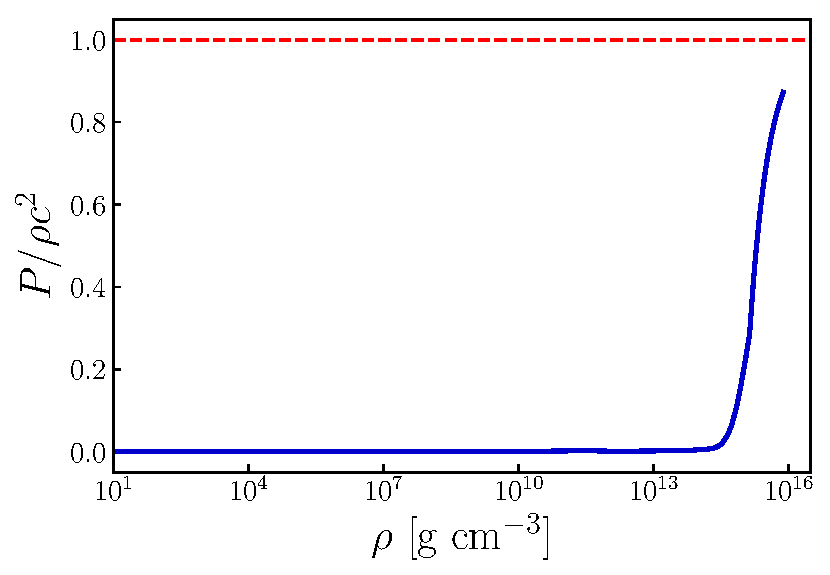
\includegraphics[width=1\textwidth]{figures/ECeng.pdf}
        \caption[Verificación de C6 para la EOS ENG]{Verificación de C6 para la EOS ENG. La línea roja punteada indica la igualdad $P=\rho c^2$. Se aprecia que $P/\rho c^2 \leq 1$, por lo que esta ecuación de estado cumple C6.}
        \label{DECeng}
    \end{minipage}
    \quad
    \begin{minipage}[b]{.48\textwidth}
        \centering
        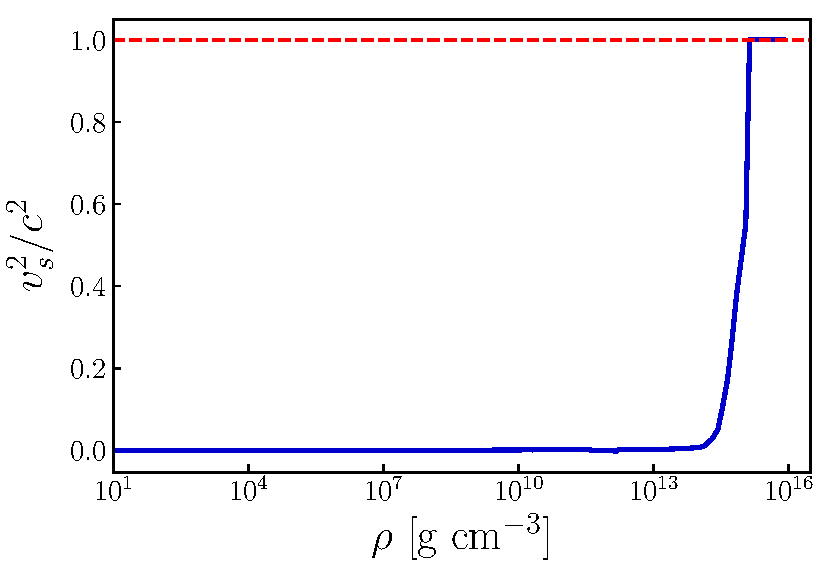
\includegraphics[width=1\textwidth]{figures/SSeng.pdf}
        \caption[Verificación de C7 para la EOS ENG]{Verificación de C7 para la EOS ENG. La línea roja punteada representa $v_s=c$. Se aprecia que $v_s^2/c^2 \leq 1$, por lo que esta ecuación de estado cumple C7.}
        \label{SSCeng}
    \end{minipage}
\end{figure}



\begin{figure}[H]
    \centering
    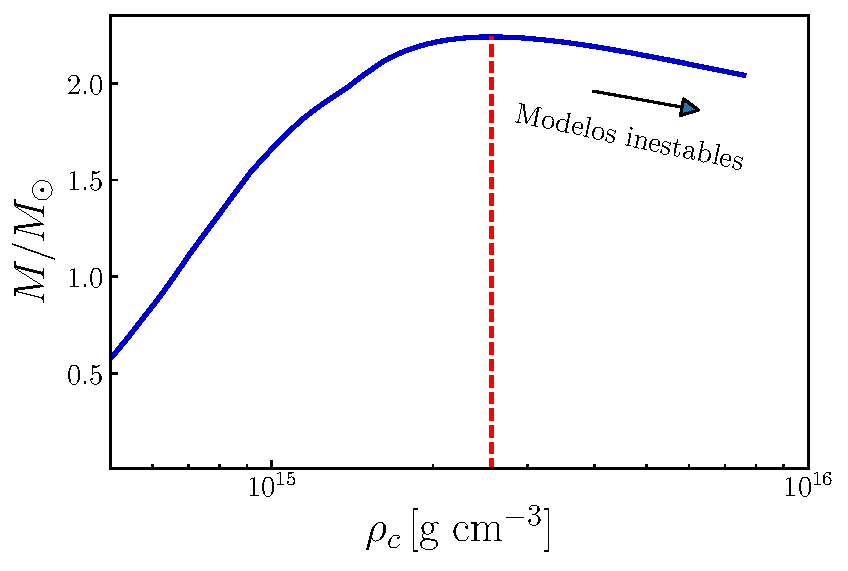
\includegraphics[width=0.7\linewidth]{figures/Mrhorel_eng.pdf}
    \caption[Identificando los modelos obtenidos con la EOS ENG que no satisfacen C10]{Identificando los modelos obtenidos con la EOS ENG que no satisfacen C10. La masa máxima para esta ecuación de estado fue $M_{max}=2.241\,M_{\odot}$ alcanzada con la densidad central $\rho_c=2.5704 \times 10^{15}$ (línea roja punteada), así que modelos con $\rho_c \geq 2.5704 \times 10^{15}$ serán inestables ante pulsaciones radiales. }
    \label{mrhoeng}
\end{figure}
%Tras confirmar que la ecuación de estado cumple C6 y C7, se procede a solucionar las ecuaciones de TOV para un conjunto de densidades centrales (valores iniciales) que típicamente va desde $\rho_c=\rho_0 \sim 10^{14} \text{g cm}^{-3}$ hasta la máxima densidad disponible en la ecuación de estado. Como por construcción las soluciones cumplen las condiciones C1,C2,C4 y C5 (como es descrito en el Apéndice \ref{NumSol}), se utiliza la condición C10 para restringir los modelos a analizar: sólo se considerarán modelos con densidades centrales tales que $\frac { \partial M \left( \rho _ { c } \right) } { \partial \rho _ { c } } > 0$. Esta derivada es nula para la configuración con masa máxima y se presenta un cambio del signo de la derivada de positiva a negativa, la densidad central para la que esto sucede indica el inicio de las configuraciones inestables (ver Figura \ref{mrhoeng}).
Para continuar con el análisis de la aceptabilidad física de los modelos que satisfacen C10, se halló la primera y segunda derivada de $\rho$ y $P$ respecto a la coordenada radial $r$ numéricamente (los detalles de cómo se obtuvo las derivadas numéricamente se encuentran en la Sección \ref{NumDer} del Apéndice \ref{NumSol}) con el objetivo de verificar las condiciones C9 y C11.  

Haciendo un análisis gráfico de $\dv{P(r)}{r} $ (ver Figura \ref{CrackStabilityeng}) se determinó que todos los modelos que satisfacen C10 también satisfacen C9. 
 

\begin{figure}[H]
    \centering
    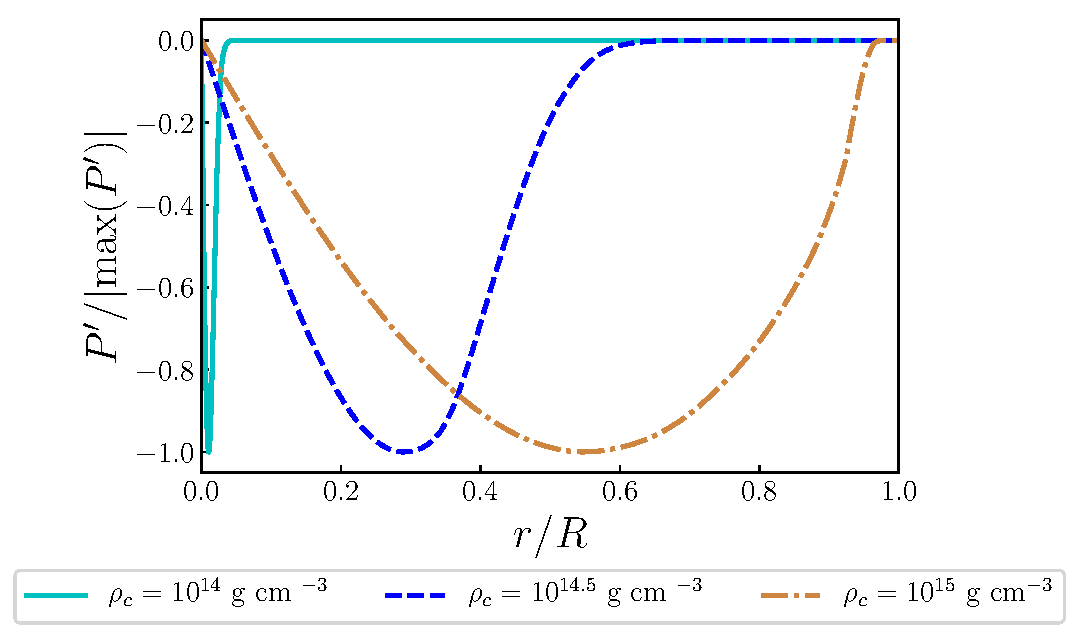
\includegraphics[width=0.93\linewidth]{figures/CrackStabilityeng.pdf}
    \caption[Verificación de C9 para la EOS ENG]{Verificación de C9 para la EOS ENG. Se presentan los gradientes de presión de una muestra representativa de los modelos que cumplen con C10. Estos siempre son menores  iguales a cero  y por lo tanto los modelos considerados son estables ante cracking si se realizan perturbaciones constantes.}
    \label{CrackStabilityeng}
\end{figure}
Por otro lado, el análisis gráfico de $\dv[2]{\rho}{r}$ reveló que en todos los modelos hay una región en la cual no se cumple la condición C11 (ver Figura \ref{ConvecStabilityeng}), esto es, hay regiones que no serían estables ante movimientos convectivos adiabáticos. Al graficar $\dv[2]{\rho}{r}$ contra $\rho$ (ver Figura \ref{ConvecStabilityengCorrel}) se identifica que la zona que no cumple la condición C11 está acotada entre densidades cercanas a $\rho_{ND}\approx 4 \times 10^{11} $ y densidades cercanas $\rho_0$ (aŕea sombreada). Este rango de densidades concuerda con las encontradas en la corteza interior (ver Figura \ref{NSS}) y sugiere que esta región hace que los modelos obtenidos con la EOS ENG sean inestables antes ante convección adiabática. En la siguiente sección se mostrará que este comportamiento está presente en todas las EOSs consideradas.
%\REMARK{¿Sí quito la figura que viene? La dejaba porque fue parte del proceso de darse cuenta.}
\begin{figure}[H]
    \centering
    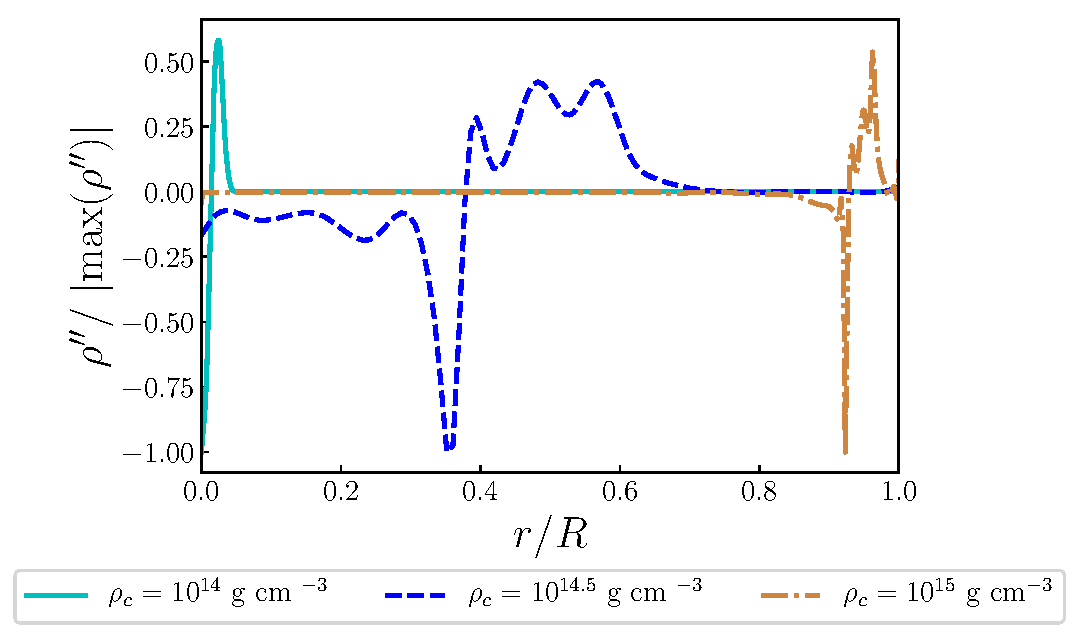
\includegraphics[width=0.93\linewidth]{figures/ConvecStabilityeng.pdf}
    \caption[Verificación de C11 para la EOS ENG]{Verificación de C11 para la EOS ENG. Se presenta $\rho^{\prime\prime}(r)$ de una muestra representativa de los modelos que cumplen con C10. La condición no se cumple en toda la estrella para todos los modelos. }
    \label{ConvecStabilityeng}
\end{figure}
\begin{figure}[H]
    \centering
    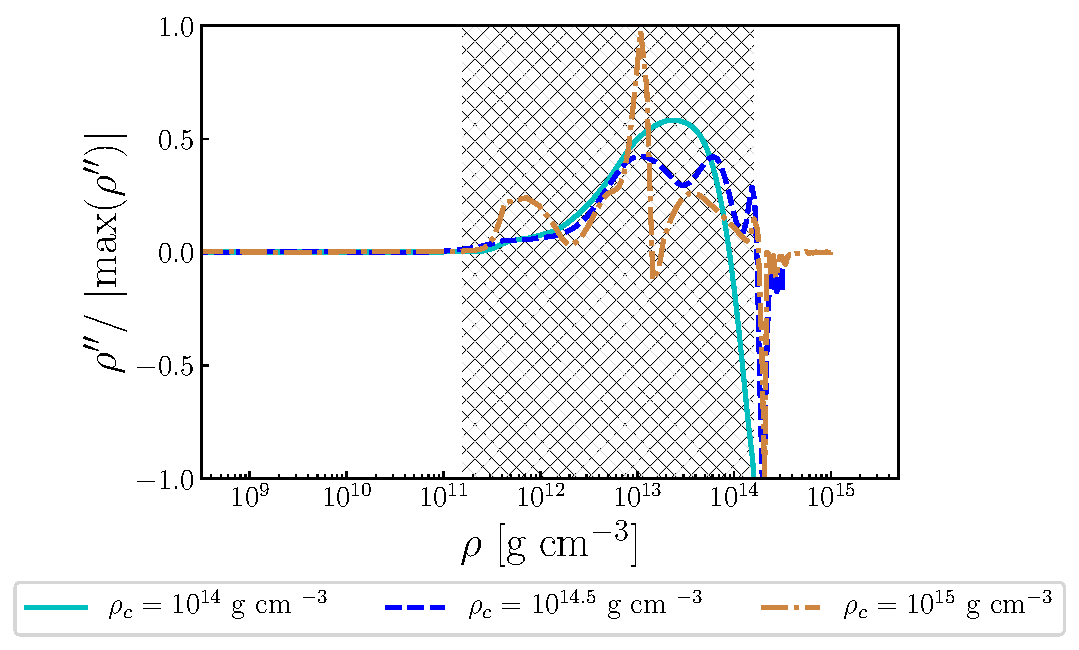
\includegraphics[width=0.93\linewidth]{figures/ConvecStabilityengCorrel.pdf}
    \caption[Correlación entre la inestabilidad y la corteza interior usando el diagrama $\rho^{\prime\prime}$ vs $\rho$]{El gráfico $\rho^{\prime\prime}(\rho)$ permite identificar la ubicación de las inestabilidades: para todos los modelos se encuentran en el rango de densidades ($\rho_{ND},\rho_0$) (área sombreada), lo que pudiera indicar que se trata de la corteza interior de la estrella.} 
    \label{ConvecStabilityengCorrel}
\end{figure}

Finalmente se verificó que los modelos considerados son consistentes con la condición C3 calculando el corrimiento al rojo como función de la coordenada radial \eqref{redshift} (ver Figura \ref{Redshifteng}). 

\begin{figure}[H]
    \centering
    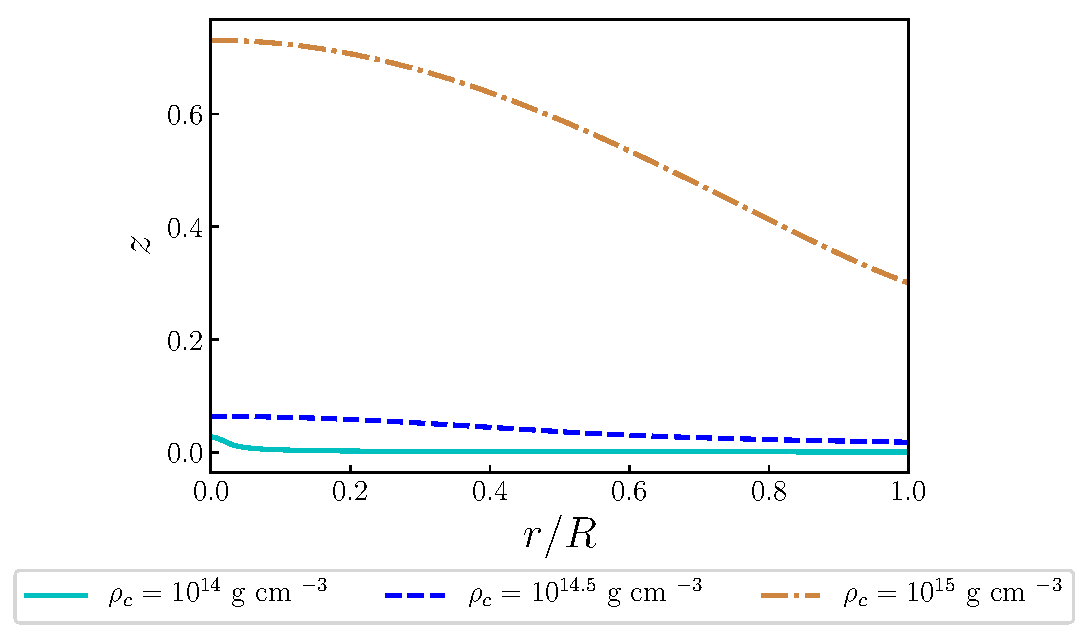
\includegraphics[width=0.93\linewidth]{figures/Redshifteng.pdf}
    \caption[Verificación de C3 para la EOS ENG]{Verificación de C3 para la EOS ENG. Se graficó el corrimiento al rojo $z$ como una función de $r$. Se aprecia que $z$ decrece alcanzando un mínimo en el borde de la estrella para los modelos considerados, satisfaciendo C3.}
    \label{Redshifteng}
\end{figure}

\section{Consolidados}

\noindent Tras realizar un análisis análogo al presentado en la sección anterior para todo el conjunto de 37 EOSs, los resultados fueron sintetizados en la Tabla \ref{Consolidados} y pueden ser consultados en el notebook de Jupyter RAnalysis \footnote{\url{https://nbviewer.jupyter.org/github/DavidRamosSal/stellar_structure/blob/master/RAnalysis.ipynb}}. En primer lugar se encontró que todas las EOSs consideradas producen modelos estelares que son estables ante cracking. Se encontró que 31 de las 37 EOSs producen modelos estelares que presentan inestabilidades convectivas en la corteza interior (comportamiento descrito en la Figura \ref{ConvecStabilityengCorrel} en el mismo rango de densidades).

Tres EOSs (H4-7) no pudieron ser evaluadas rigurosamente pues las tablas sólo contenían la parte más densa de la EOS ($\rho > 10^{14}$), presuntamente para ser acoplada posteriormente con una EOS para la corteza y por lo tanto no se pudo evaluar la estabilidad convectiva en esta región. Finalmente, para tres EOSs (SQM1-3) se encontró que los modelos producidos son inestables ante convección adiabática sólo cerca a la superficie. Como la región en la que se presentan las inestabilidades corresponde a un rango de densidades cercano al borde de la estrella, puede deberse a un error numérico.

Los valores de $M_{\text{max}}$ y el respectivo radio $R_{M_{\text{max}}}$ calculados para cada EOS son cercanos a los obtenidos en \cite{Read2009} para un conjunto similar de EOSs y representan por lo tanto otra forma de validar los cálculos. Sin embargo, como este trabajo está orientado al análisis de los perfiles de densidad y presión, no se procederá a calcular diferencias para estos parámetros entre las dos simulaciones. 

\begin{table}[H]
\caption[Resultados consolidados]{Resultados para las 37 EOSs consideradas. C3: corrimiento al rojo, C6: condición de energía dominante, C7: causalidad, C9: cracking, C11: movimientos convectivos. Se listan además el método teórico usado para obtener la EOS, los componentes que interactúan fuertemente (todos los modelos incluyen contribuciones leptónicas), la masa máxima $M_{\text{max}}$ y el respectivo radio $R_{M_{\text{max}}}$ para estrellas estáticas y la referencia a los trabajos originales.}
\label{Consolidados}
\begin{adjustbox}{max width=\textwidth}
\begin{tabular}{ccccccccccc}
\hline
\multirow{2}{*}{\textbf{EOS}} & \multirow{2}{*}{\textbf{Método}}           & \multirow{2}{*}{\textbf{Composición}} & \multirow{2}{*}{\begin{tabular}[c]{@{}c@{}}$\mathbf{M}_{\text{\textbf{max}}}$\\  $[\mathbf{M_{\odot}}]$\end{tabular}} & \multirow{2}{*}{\begin{tabular}[c]{@{}c@{}}$\mathbf{R}_{\mathbf{M}_{\text{\textbf{max}}}}$\\  $[$\textbf{km}$]$\end{tabular}} & \multirow{2}{*}{\textbf{C3}} & \multirow{2}{*}{\textbf{C6}} & \multirow{2}{*}{\textbf{C7}} & \multirow{2}{*}{\textbf{C9}} & \multirow{2}{*}{\textbf{C11}} & \multirow{2}{*}{\textbf{Referencia}}          \\
                     &                                   &                              &                                                                                            &                                                                                           &                     &                     &                     &                     &                      &                                      \\ \hline \addlinespace
ALF1                 & \multirow{4}{*}{Mixto}            & \multirow{4}{*}{$n,p,q$}     & 1.496                                                                                      & 9.221                                                                                     & \checkmark          & \checkmark          & \checkmark          & \checkmark          & \Cross               & \multirow{4}{*}{\cite{Alford2005}}   \\
ALF2                 &                                   &                              & 2.087                                                                                      & 11.962                                                                                    & \checkmark          & \checkmark          & \checkmark          & \checkmark          & \Cross               &                                      \\
ALF3                 &                                   &                              & 1.473                                                                                      & 9.514                                                                                     & \checkmark          & \checkmark          & \checkmark          & \checkmark          & \Cross               &                                      \\
ALF4                 &                                   &                              & 1.943                                                                                      & 10.892                                                                                    & \checkmark          & \checkmark          & \checkmark          & \checkmark          & \Cross               &                                      \\ \addlinespace
AP1                  & \multirow{4}{*}{Variacional}      & \multirow{4}{*}{$n,p$}       & 1.684                                                                                      & 8.292                                                                                     & \checkmark          & \checkmark          & \checkmark          & \checkmark          & \Cross               & \multirow{4}{*}{\cite{Akmal1998}}    \\
AP2                  &                                   &                              & 1.809                                                                                      & 8.746                                                                                     & \checkmark          & \checkmark          & \Cross              & \checkmark          & \Cross               &                                      \\
AP3                  &                                   &                              & 2.391                                                                                      & 10.765                                                                                    & \checkmark          & \Cross              & \Cross              & \checkmark          & \Cross               &                                      \\
AP4                  &                                   &                              & 2.214                                                                                      & 10.004                                                                                    & \checkmark          & \Cross              & \Cross              & \checkmark          & \Cross               &                                      \\ \addlinespace
BBB2                 & BD-HF                     & $n,p$                        & 1.920                                                                                      & 9.515                                                                                     & \checkmark          & \checkmark          & \checkmark          & \checkmark          & \Cross               & \cite{Lombardo2004}                  \\ \addlinespace
BGN1H1               & Potencial efectivo                & $n,p,H$                      & 1.630                                                                                      & 9.325                                                                                     & \checkmark          & \checkmark          & \checkmark          & \checkmark          & \Cross               & \cite{Balberg1997}                   \\ \addlinespace
BPAL12               & BD-HF                     & $n,p$                        & 1.455                                                                                      & 9.015                                                                                     & \checkmark          & \checkmark          & \checkmark          & \checkmark          & \Cross               & \cite{Zuo1999}                       \\ \addlinespace
BSK19                & \multirow{3}{*}{Potencial efectivo}              & \multirow{3}{*}{$n,p$}       & 1.861                                                                                      & 9.110                                                                                     & \checkmark          & \Cross              & \Cross              & \checkmark          & \Cross               & \multirow{3}{*}{\cite{Potekhin2013}} \\
BSK20                &                                   &                              & 2.165                                                                                      & 10.173                                                                                    & \checkmark          & \Cross              & \Cross              & \checkmark          & \Cross               &                                      \\
BSK21                &                                   &                              & 2.274                                                                                      & 11.038                                                                                    & \checkmark          & \Cross              & \Cross              & \checkmark          & \Cross               &                                      \\ \addlinespace
ENG                  & BD-HF                     & $n,p$                        & 2.241                                                                                      & 10.425                                                                                    & \checkmark          & \checkmark          & \checkmark          & \checkmark          & \Cross               & \cite{Engvik1994}                    \\ \addlinespace
FPS                  & Variacional                       & $n,p$                        & 1.800                                                                                      & 9.279                                                                                     & \checkmark          & \checkmark          & \checkmark          & \checkmark          & \Cross               & \cite{Friedman1981}                  \\ \addlinespace
GNH3                 & Teoría de campos                  & $n,p,H,\Delta$               & 1.965                                                                                      & 11.372                                                                                    & \checkmark          & \checkmark          & \checkmark          & \checkmark          & \Cross               & \cite{Glendenning1985}               \\ \addlinespace
H1                   & \multirow{6}{*}{Teoría de campos} & \multirow{6}{*}{$n,p,H$}     & 1.556                                                                                      & 10.968                                                                                    & \checkmark          & \checkmark          & \checkmark          & \checkmark          & \Cross               & \multirow{6}{*}{\cite{Lackey2006}}   \\
H2                   &                                   &                              & 1.668                                                                                      & 11.516                                                                                    & \checkmark          & \checkmark          & \checkmark          & \checkmark          & \Cross               &                                      \\
H3                   &                                   &                              & 1.790                                                                                      & 11.863                                                                                    & \checkmark          & \checkmark          & \checkmark          & \checkmark          & \Cross               &                                      \\
H4                   &                                   &                              & 2.032                                                                                      & 11.467                                                                                    & \checkmark          & \checkmark          & \checkmark          & \checkmark          & -           &                                      \\
H5                   &                                   &                              & 1.726                                                                                      & 10.930                                                                                    & \checkmark          & \checkmark          & \checkmark          & \checkmark          &  -           &                                      \\
H7                   &                                   &                              & 1.683                                                                                      & 10.474                                                                                    & \checkmark          & \checkmark          & \checkmark          & \checkmark          & -           &                                      \\ \addlinespace
MPA1                 & BD-HF                     & $n,p$                        & 2.462                                                                                      & 11.301                                                                                    & \checkmark          & \checkmark          & \checkmark          & \checkmark          & \Cross               & \cite{Muther1987}                    \\ \addlinespace
 \hline \addlinespace
\multicolumn{1}{l}{} & \multicolumn{1}{l}{}              & \multicolumn{1}{l}{}         & \multicolumn{1}{l}{}                                                                       & \multicolumn{1}{l}{}                                                                      & \multicolumn{1}{l}{} & \multicolumn{1}{l}{} & \multicolumn{4}{l}{\small{(Continúa en la siguiente página)}} 
\end{tabular}
\end{adjustbox}
\end{table}


% Please add the following required packages to your document preamble:
% \usepackage{multirow}
\begin{table}[H]
\renewcommand\thetable{3.1 (continuación)}
\caption[]{}
\begin{adjustbox}{max width=\textwidth}
\begin{tabular}{ccccccccccc}
\hline
\multirow{2}{*}{\textbf{EOS}} & \multirow{2}{*}{\textbf{Método}}           & \multirow{2}{*}{\textbf{Composición}} & \multirow{2}{*}{\begin{tabular}[c]{@{}c@{}}$\mathbf{M}_{\text{\textbf{max}}}$\\  $[\mathbf{M_{\odot}}]$\end{tabular}} & \multirow{2}{*}{\begin{tabular}[c]{@{}c@{}}$\mathbf{R}_{\mathbf{M}_{\text{\textbf{max}}}}$\\  $[$\textbf{km}$]$\end{tabular}} & \multirow{2}{*}{\textbf{C3}} & \multirow{2}{*}{\textbf{C6}} & \multirow{2}{*}{\textbf{C7}} & \multirow{2}{*}{\textbf{C9}} & \multirow{2}{*}{\textbf{C11}} & \multirow{2}{*}{\textbf{Referencia}}          \\
                     &                                   &                              &                                                                                            &                                                                                           &                     &                     &                     &                     &                      &                                      \\ \hline \addlinespace
MS1                  & \multirow{2}{*}{Teoría de campos} & \multirow{2}{*}{$n,p$}       & 2.770                                                                                      & 13.346                                                                                    & \checkmark          & \checkmark          & \checkmark          & \checkmark          & \Cross               & \multirow{2}{*}{\cite{Muller1996}}   \\
MS1b                 &                                   &                              & 2.778                                                                                      & 13.301                                                                                    & \checkmark          & \checkmark          & \checkmark          & \checkmark          & \Cross               &                                      \\ \addlinespace
NL3                  & Teoría de campos                  & $n,p,\sigma,\omega,\rho$     & 2.806                                                                                      & 13.427                                                                                    & \checkmark          & \checkmark          & \checkmark          & \checkmark          & \Cross               & \cite{Lalazissis1997}                \\ \addlinespace
PAL6                 & Potencial esquemático                             & $n,p$                        & 1.478                                                                                      & 9.258                                                                                     & \checkmark          & \checkmark          & \checkmark          & \checkmark          & \Cross               & \cite{Prakash1988}                   \\ \addlinespace
PCL2                 & Teoría de campos                  & $n,p,H,q$                    & 1.483                                                                                      & 10.116                                                                                    & \checkmark          & \checkmark          & \checkmark          & \checkmark          & \Cross               & \cite{Prakash1995}                   \\ \addlinespace
PS                   & Teoría de campos                  & $n,\pi^0$                    & 1.755                                                                                      & 11.372                                                                                    & \checkmark          & \checkmark          & \checkmark          & \checkmark          & \Cross               & \cite{Pandharipande1975}             \\ \addlinespace
SLy                  & Mixto                             & $n,p$                        & 2.050                                                                                      & 9.977                                                                                     & \checkmark          & \checkmark          & \Cross              & \checkmark          & \Cross               & \cite{Douchin2001}                   \\ \addlinespace
SQM1                 & \multirow{3}{*}{Teoría de campos} & \multirow{3}{*}{$q$}         & 1.532                                                                                      & 8.315                                                                                     & \checkmark          & \checkmark          & \checkmark          & \checkmark          & -*                    & \multirow{3}{*}{\cite{Prakash1995}}  \\
SQM2                 &                                   &                              & 1.737                                                                                      & 9.638                                                                                     & \checkmark          & \checkmark          & \checkmark          & \checkmark          & -*                    &                                      \\
SQM3                 &                                   &                              & 1.977                                                                                      & 10.814                                                                                    & \checkmark          & \checkmark          & \checkmark          & \checkmark          & -*                    &                                      \\ \addlinespace
WFF1                 & \multirow{3}{*}{Variacional}      & \multirow{3}{*}{$n,p$}       & 2.134                                                                                      & 9.413                                                                                     & \checkmark          & \checkmark          & \Cross              & \checkmark          & \Cross               & \multirow{3}{*}{\cite{Wiringa1988}}  \\
WFF2                 &                                   &                              & 2.199                                                                                      & 9.825                                                                                     & \checkmark          & \checkmark          & \Cross              & \checkmark          & \Cross               &                                      \\
WFF3                 &                                   &                              & 1.845                                                                                      & 9.516                                                                                     & \checkmark          & \checkmark          & \checkmark          & \checkmark          & \Cross               &                                      \\ \addlinespace \hline \addlinespace
\multicolumn{3}{l}{\small{*Resultados con problemas en la frontera}}                                            & \multicolumn{1}{l}{}                                                                       & \multicolumn{1}{l}{}                                                                      & \multicolumn{1}{l}{} & \multicolumn{1}{l}{} & \multicolumn{1}{l}{} & \multicolumn{1}{l}{} & \multicolumn{1}{l}{} & \multicolumn{1}{l}{}             
\end{tabular}
\end{adjustbox}
\end{table}

\section{Discusión}

\noindent A continuación se presentará una discusión sobre los resultados encontrados para las condiciones de aceptabilidad evaluada.

\emph{C3: corrimiento al rojo}. A pesar de que el valor del corrimiento al rojo gravitacional $z$ en la superficie sea muy sensible a la EOS utilizada (por estar relacionado con la masa y el radio de la estrella), se encontró que el comportamiento de $z$ como función de la coordenada $r$ no varía entre las EOSs: decrece monótonamente del centro al borde de la esfera satisfaciendo la condición de aceptabilidad y aumenta globalmente con la densidad central (Figura \ref{Redshifteng}).

\emph{C6: condición de energía dominante} y \emph{C7: Causalidad}. Tras encontrar que EOSs usadas ampliamente en aplicaciones no cumplen estas condiciones surge la pregunta: ¿puede una EOS físicamente correcta violar C6 y C7? De acuerdo a \cite{Haensel2007} existen ejemplos de modelos que a pesar de no cumplir C6 y C7 siguen siendo causales e invariantes ante transformaciones de Lorentz. Sin embargo, el hecho de que los modelos que no cumplen estas condiciones están basados en esquemas de muchos cuerpos no relativistas sugiere que los modelos son artificiales pues este tipo de comportamientos no se presenta en esquemas relativistas. Además, se encontró que todas las ecuaciones que no cumplen C6 tampoco cumplen C7, mientras que lo opuesto no se cumple, esto sugiere que otras características aparte de la rigidez de la EOS pueden resultar en violaciones a C7. Por otro lado se ha sugerido que la condición C7 se debe cumplir sólo a densidades realizables en las estrellas de neutrones \cite{Douchin2001}, esto es, a densidades menores a la densidad para la que se obtiene la masa máxima. Si esto es correcto, algunas de las EOS que cumplen C6 pero no C7 seguirían siendo físicamente aceptables, pero no se intentará resolver ese problema en este trabajo.

\emph{C9: cracking}. Se confirmó que todos los modelos son estables ante cracking para el caso de perturbaciiones constantes, este resultado era esperado por tratarse de soluciones de fluido perfecto y se había obtenido para otras soluciones de fluido perfecto como la Tolman VI \cite{Herrera1992}.

\emph{C11: convección adiabática}. Los resultados indican que según el criterio C11 la corteza interior de las estrellas de neutrones es inestable ante convección, para todas las EOSs consideradas. Previamente en \cite{Miralles1997} se mostró que en estrellas débilmente magnetizadas, la envoltura de la estrella de neutrones puede ser inestable ante convección. Sin embargo, nada se ha reportado acerca de la estabilidad de la corteza interior. Es sabido \cite{Haensel2007} que las transiciones de fase primer orden que ocurren en la interfaz corteza-núcleo producen discontinuidades en el perfil de densidad, esto es observado en los resultados (pico en regiones con densidades cercanas a $\rho_0$ en la Figura \ref{ConvecStabilityengCorrel}) y puede tener algo que ver con la existencia de la inestabilidad en regiones que se acercan a estas densidades.

\vspace{0.3cm}
\noindent\textbf{Sobre el criterio de estabilidad C8}

\begin{figure}[H]
    \centering
    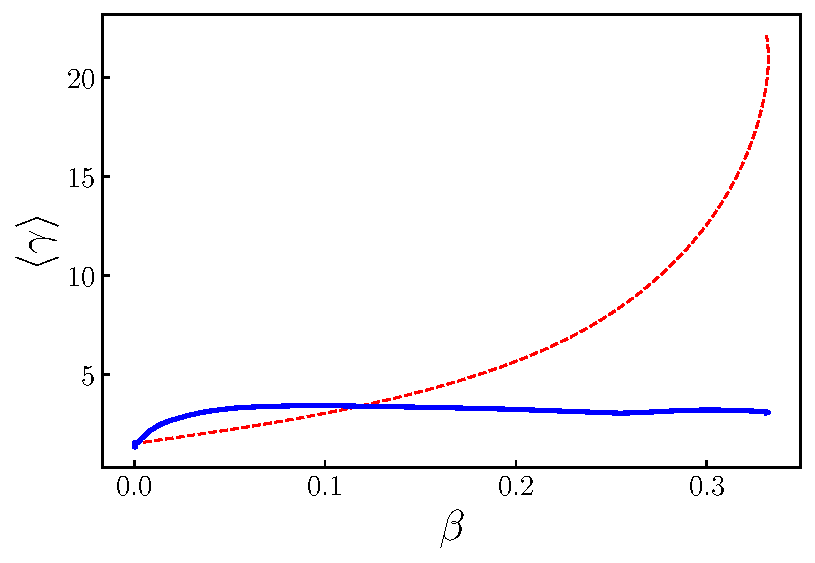
\includegraphics[width=0.6\linewidth]{figures/AdiabaticIndexENGbeta.pdf}
    \caption[Estabilidad usando el índice adiabático]{Verificación de C8 para la EOS ENG. La línea roja punteada representa $\gamma_{cr}$. La igualdad $\langle \gamma \rangle$ no se alcanza para la compacidad de la configuración de masa máxima ($\beta_{cr}=0.317$ en este caso) como es presentado en \cite{Koliogiannis2019a}, debido al rápido crecimiento de $\gamma_{cr}$.} 
    \label{AdiabaticIndexCriterio}
\end{figure}

\noindent Recientemente \cite{Koliogiannis2019a} se usó la restricción que impone este criterio sobre el índice adiabático efectivo $\langle \gamma \rangle$ para obtener una relación entre la compacidad de la configuración con masa máxima $\beta_{cr}$ y el índice adiabático $\gamma_{cr}$, que es independiente de la EOS. Sin embargo, los resultados encontrados arrojan un crecimiento muy rápido $\gamma_cr$ con la compacidad $\beta$ para todas las EOSs (ver la Figura \ref{AdiabaticIndexCriterio} para un ejemplo) que no predice la igualdad $\langle \gamma \rangle = \gamma_{cr}$ para el valor de $\beta_{cr}$.

Este resultado es preliminar y se espera verificar que las integrales presentes en el cálculo de $\gamma_{cr}$ \eqref{gammacrit} no estén introduciendo un error numérico.